\documentclass[tikz,border=10pt]{standalone}
\usepackage{amsmath}

\begin{document}

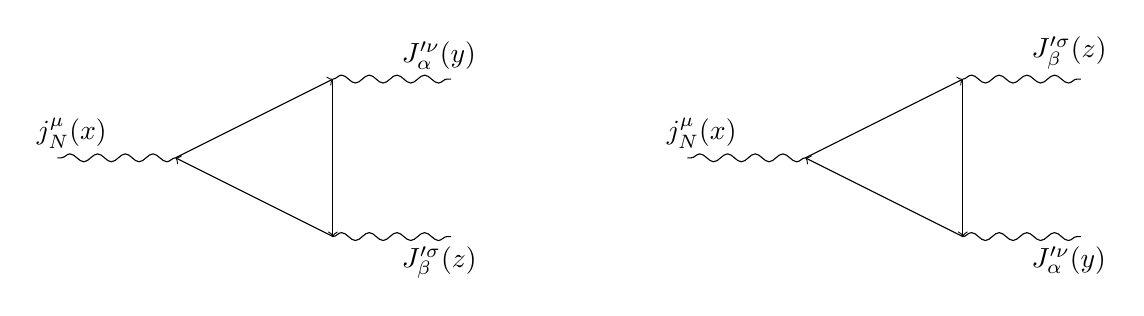
\begin{tikzpicture}

% First diagram
\begin{scope}[xshift=-4cm]
    % Axes
    \coordinate (A) at (0,0);
    \coordinate (B) at (2,1);
    \coordinate (C) at (2,-1);
    
    % Lines
    \draw[decorate, decoration={snake, amplitude=.5mm}] (A) -- node[midway, above left] {$j_N^{\mu}(x)$} ++(-1.5,0);
    \draw[->] (A) -- (B) node[midway, above right] {};
    \draw[->] (B) -- (C) node[midway, right] {};
    \draw[->] (C) -- (A) node[midway, below right] {};
    \draw[decorate, decoration={snake, amplitude=.5mm}] (B) -- node[midway, above right] {$J'^\nu_\alpha(y)$} ++(1.5,0);
    \draw[decorate, decoration={snake, amplitude=.5mm}] (C) -- node[midway, below right] {$J'^\sigma_\beta(z)$} ++(1.5,0);
\end{scope}

% Second diagram
\begin{scope}[xshift=4cm]
    % Axes
    \coordinate (A) at (0,0);
    \coordinate (B) at (2,1);
    \coordinate (C) at (2,-1);
    
    % Lines
    \draw[decorate, decoration={snake, amplitude=.5mm}] (A) -- node[midway, above left] {$j_N^{\mu}(x)$} ++(-1.5,0);
    \draw[->] (A) -- (B) node[midway, above right] {};
    \draw[->] (B) -- (C) node[midway, right] {};
    \draw[->] (C) -- (A) node[midway, below right] {};
    \draw[decorate, decoration={snake, amplitude=.5mm}] (B) -- node[midway, above right] {$J'^\sigma_\beta(z)$} ++(1.5,0);
    \draw[decorate, decoration={snake, amplitude=.5mm}] (C) -- node[midway, below right] {$J'^\nu_\alpha(y)$} ++(1.5,0);
\end{scope}

\end{tikzpicture}

\end{document}